%!TEX root = ../../report.tex
\clearpage
\subsection{Deployment View}
This subsection outlinesshow the physical arrangement of the nodes in a distributed system, the artifacts that are stored on each node, and the components and other elements that the artifacts implement \cite{ibmdeployment}. Communication paths and deploy relationships model the connections in the system.

\subsubsection{Deployment Diagram}
Figure \ref{fig:deployment-diagram} shows the deployment diagram of the SFM. The diagram contains several components such as, sensors, analytics cluster, and database clusters. Main communication between components are done using TCP/IP. All hardware decision are based on chapter 6.

\begin{figure}[hb!]
\centering
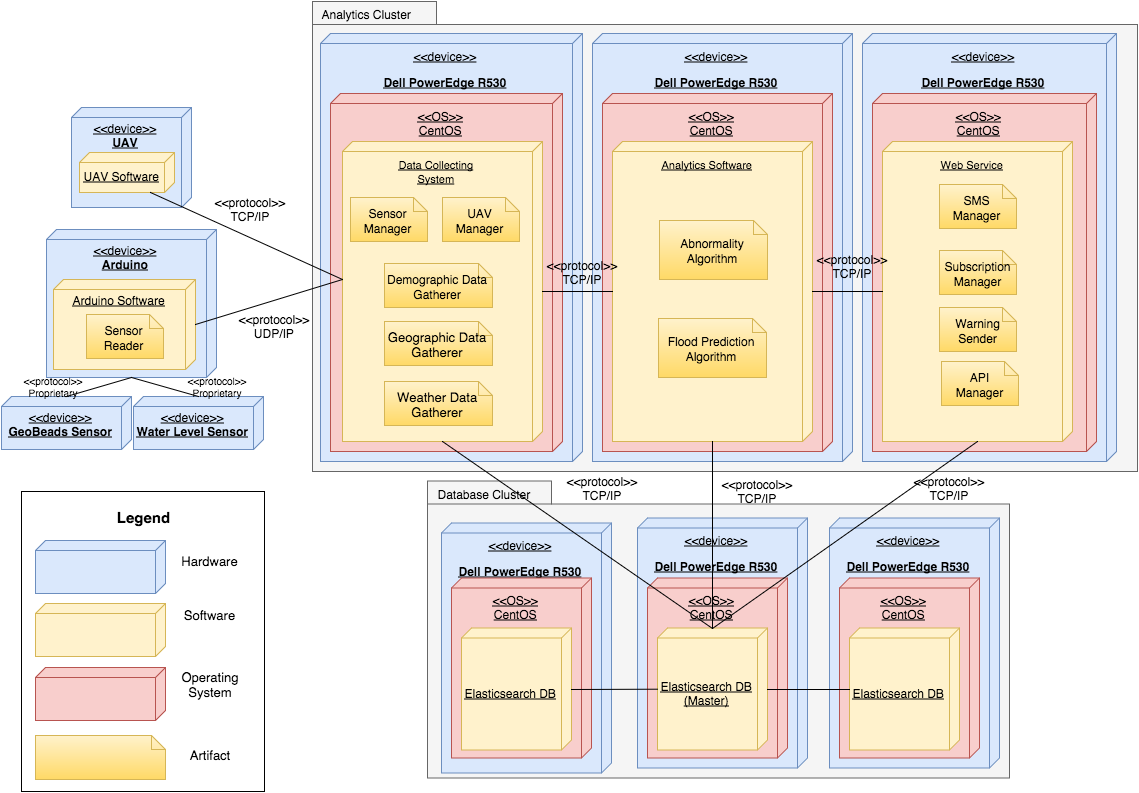
\includegraphics[keepaspectratio=true,width=1.0\textwidth]{{\viewimages/deployment-view}.pdf}
\caption{Deployment diagram}
\label{fig:deployment-diagram}
\end{figure}


% To-Do:
% Artifacts